%
% this file is encoded in utf-8
% v2.0 (Apr. 5, 2009)

\documentclass[12pt, a4paper]{ntuthesis}

% 除非校方修改了論文格式 (margins, header, footer, 浮水印, 中文數字之章別)
% 或者需要增加所用的 LaTeX 套件,
% 或者要改預設中文字型、編碼
% 否則毋須修改本檔內容
% 論文撰寫,請修改以 my_  開頭檔名的各檔案

\usepackage{CJKutf8}  %%% ZZZ %%% macro for Chinese/Japanese/Korean processing
\usepackage{CJKnumb} %%% ZZZ %%% for Chinese numbering capability
\usepackage[nospace]{cite}  % for smart citation
%\usepackage{geometry}  % for easy margin settings
\usepackage{ntuthesis}
\usepackage{multirow,multicol,rotating}

%
% margins setting
%\geometry{verbose,a4paper,tmargin=3.5cm,bmargin=2cm,lmargin=4cm,rmargin=2cm}
%

% 插圖套件 graphicx
% 使用者工作流程是用 pdftex 還是 latex + dvipdfmx?
% 視情況而有不同的參數
% 這裡作自動判斷
% 參考自
% http://www.tex.ac.uk/cgi-bin/texfaq2html?label=ifpdf
\newcommand\mydvipdfmxflow{dvipdfmx}
\newcommand\mypdftexflow{pdftex}
\ifx\pdfoutput\undefined
  % not running pdftex
  \usepackage[dvipdfm]{graphicx}
  \newcommand\myworkflow{dvipdfmx}  % set the flag for hyperref
\else
  \ifx\pdfoutput\relax
    % not running pdftex
    \usepackage[dvipdfm]{graphicx}
    \newcommand\myworkflow{dvipdfmx}  % set the flag
  \else
    % running pdftex, with...
    \ifnum\pdfoutput>0
      % ... PDF output
      %\usepackage[pdftex]{graphicx}
      \newcommand\myworkflow{pdftex}  % set the flag
    \else
      %...DVI output
      \usepackage[dvipdfm]{graphicx}
      \newcommand\myworkflow{dvipdfmx}  % set the flag
    \fi
  \fi
\fi

% 增強功能型頁楣 / 頁腳套件
\usepackage{fancyhdr}  % 借用此套件來擺放浮水印 
% (佔用了 central header)
% 不需要浮水印的使用者仍可利用此套件,產生所需的 header, footer
%
% 啟動 fancy header/footer 套件
\pagestyle{fancy}
\fancyhead{}  % reset left, central, right header to empty
\fancyfoot[C]{\thepage} %中間 footer 擺放頁碼
\renewcommand{\headrulewidth}{0pt} % header 的直線; 0pt 則無線

% 如果不需要任何浮水印,則請把下列介於 >>> 與 <<< 之間
% 的文字行關掉 (行首加上百分號)
%% 浮水印 >>> 
%\input{yzu_watermark.tex}
%% <<< 浮水印

% 如需額外的頁楣 (header) 或 footer,請在 my_headerfooter.tex 裡依例修改
% 它的預設內容是都關掉,可依需要打開
\input{my_headerfooter.tex}



%%%%%%%%%%%%%%%%%%%%%%%%%%%%%%
%%%% 非必要的套件,但很實用
\usepackage{amsmath} % 各式 AMS 數學功能
\usepackage{amssymb} % 各式 AMS 數學符號
\usepackage{mathrsfs} %草寫體數學符號,在數學模式裡用 \mathscr{E} 得草寫 E
\usepackage{listings} % 程式列表套件
\usepackage{subfig}
\usepackage{tabularx}
\usepackage{url}
\usepackage[usenames,dvipsnames]{xcolor}
\usepackage{pgf}
\usepackage{tikz}
\usetikzlibrary{arrows,automata,positioning}



% Title Page
\renewcommand{\enTitle}{Question Answering}  %英文標題
\renewcommand{\zhTitle}{問答}  %中文標題
\renewcommand{\authorZhName}{吳柏瑜}  %作者中文姓名
\renewcommand{\authorEnName}{Wu Po-Yu}  %作者英文姓名
\renewcommand{\authorStudentID}{R04921034}  %作者學號
\renewcommand{\advisorZhName}{李宏毅}  %指導教授中文姓名
\renewcommand{\advisorEnName}{Hung-yi Lee}  %指導教授英文姓名
\renewcommand{\zhCollegeName}{電機資訊學院}  %學院中文名稱
\renewcommand{\enCollegeName}{College of Electrical Engineering and Computer Science}  %學院英文名稱
\renewcommand{\zhDepartmentName}{電信工程學研究所}  %系所中文名稱
\renewcommand{\enDepartmentName}{Graduate Institute of Communication Engineering}  %系所英文名稱
\renewcommand{\rocYear}{一百零六}  %中華民國紀年年份
\renewcommand{\zhMonth}{六}  %中文月份
\renewcommand{\enYear}{2017}  %公元紀年
\renewcommand{\enMonth}{June}  %英文月份
\renewcommand{\oralDate}{103 年 6 月 23 日}  %口試日期

%
% listing setting
\lstset{breaklines=true,% 過長的程式行可斷行
extendedchars=false,% 中文處理不需要 extendedchars
texcl=true,% 中文註解需要有 TeX 處理過的 comment line, 所以設成 true
comment=[l]\%\%,% 以雙「百分號」做為程式中文註解的起頭標記,配合 MATLAB
basicstyle=\small,% 小號字體, 約 10 pt 大小
commentstyle=\upshape,% 預設是斜體字,會影響註解裏的英文,改用正體
%language=Octave % 會將一些 octave 指令以粗體顯示
}

\usepackage{url} % 在文稿中引用網址,可以用 \url{http://www.yzu.edu.tw} 方式

%%%% 以上為非必要套件
%%%%%%%%%%%%%%%%%%%%%%%%%%%%%%

%%% 以下是 hyperref 套件
%%%%%%%%%%%%%%%%%%%%%%%%%%%%%%
% hyperref 會擾亂 cite.sty 對文獻號碼縮編的排版,所以依據
% http://www.ctan.org/tex-archive/macros/latex/contrib/hyperref/
% 作如下的更動,使得 hyperref 不做文獻號碼的超連結。
\makeatletter
\def\NAT@parse{\typeout{This is a fake Natbib command to fool Hyperref.}}
\makeatother

% hyperlinkable table of contents
% 章節目錄、圖表超連結
\ifx\myworkflow\mydvipdfmxflow
	\usepackage[dvipdfmx, debug, colorlinks, linkcolor=black, citecolor=black, urlcolor=black, unicode]{hyperref}
\else
	\usepackage[pdftex, debug, colorlinks, linkcolor=black, citecolor=black, urlcolor=black, unicode]{hyperref}	
\fi

% if hyperref is not used (e.g., in LyX application)
% define dummy \phantomsection for those occurences
%   in yzu_frontpages.tex, yzu_backpages.tex, my_appendix.tex
\ifx\hypersetup\undefined
	\newcommand\phantomsection{}
\fi

% hyperref跟algorithm衝突,hyperref必須放在algorithm前面
\usepackage{algorithm}
\usepackage{algorithmic}
%%%% 以上為所有套件
%%%% 
%%%% 

% global page layout
%\newcommand{\mybaselinestretch}{1.5}  %行距 1.5 倍 + 20%, (約為 double space)
%\renewcommand{\baselinestretch}{\mybaselinestretch}  % 論文行距預設值
%\parskip=2ex  % 段落之間的間隔為兩個 x 的高度
%\parindent = 0Pt  % 段首內縮由 CJK 控制,所以這裡就設成不內縮

%%%%%%%%%%%%%%%%%%%%%%%%%%%%%
%  end of preamble
%%%%%%%%%%%%%%%%%%%%%%%%%%%%%
%
\begin{document}
\begin{CJK}{UTF8}{bsmi}   %%% ZZZ %%%  <<< 在這裡更改預設中文字型、編碼
% 編碼:UTF8, Bg5, ...
% 中文字型名稱:TeXLive 安裝有一套明體字 bsmi, 楷書與其他字型視你的 LaTeX CJK 系統裝設情況而定

% 針對 latex + dvipdfmx 工作流程在 hyperref 套件的影響下,圖檔的辨識力退化
% 所作的權宜措施。可能是因為 TeXLive2007 hyperref 裏的
% 客製 graphicx / dvipdfmx 的設定檔不夠新
\ifx\myworkflow\mydvipdfmxflow
	\DeclareGraphicsExtensions{.pdf,.png,.jpg,.eps}
	\DeclareGraphicsRule{.pdf}{eps}{.bb}{}
	\DeclareGraphicsRule{.png}{eps}{.bb}{}
	\DeclareGraphicsRule{.jpg}{eps}{.bb}{}
\fi

% global CJK setting
\CJKindent  %%% ZZZ %%%  段首內縮兩格

% 載入中文名詞的定義:例如,Figure -->「圖」, Chapter -->「第 x 章」
\input{ntu_definitions.tex}

% 如果不需要以中文數字一、二、三呈現章別,例如「第一章」
% 則請把下列介於 >>> 與 <<< 之間
% 的文字行關掉 (行首加上百分號), 會以「第 1 章」呈現
%% 中文數字章別 >>>
\input{ntu_chnum.tex}
%% <<< 中文數字章別

%%% 以下是載入前頁、本文、後頁
% 請勿更動
% 如需針對個別章節獨立編譯
% 請在 my_chapters.tex 檔裡對個別章節的 \input 指令以行首百分號方式做開關。

\NTUtitlepage  % 產生論文封面

\newpage
\setcounter{page}{1}
\pagenumbering{roman}

\NTUoralpage  % 產生口試委員會審定書

\mydoublespacing
\begin{acknowledgement} %誌謝
    To Be Continued
\end{acknowledgement}

\begin{zhAbstract}  %中文摘要
    To Be Continued
\end{zhAbstract}

{
%\zhKaiFont
\mysinglespacing\selectfont
\tableofcontents %目錄

\listoffigures  %圖目錄

\listoftables  %表目錄
\par
}

\newpage
\setcounter{page}{1}
\pagenumbering{arabic}


\chapter{導論}
  \section{研究動機}
隨著科技的發展,我們越來越期望機器能夠理解問題並給予答案,進而解決一些生活上的事情。因此,我們需要一套問答系統 (Question Answering System) 來幫助我們快速的瀏覽資訊,並從中獲取答案。在過去有許多幫助我們回答問題,被開發出來並應用於產業中,如 Google Now 、Wolfram Alpha、Apple Siri等。
近年來隨著科技與網際網路的興起,維基百科 (Wikipedia) 等參考工具書正蓬勃地增加,人們追求更加直覺、便捷、有效率的資訊獲得途徑。在資料量大增的情況下,問答系統從大量的資料中直接擷取使用者想要的答案,僅只提供給使用者問題相關的答案,更加速了使用者獲得資訊的效率,因此如何讓機器能夠這些資料、理解、並回答問題,省去人們需要閱讀的時間,變成為重要的議題,而這即為問答系統。相較於其他的自然語言處理是提供給使用者文章、資源等,而問答系統有更困難的挑戰,如知識庫的廣大等,使得此問題更形艱辛。

近幾年更由於智慧型手機、穿戴式裝置的崛起與使用者需要在這些裝置上取得資訊的強烈需求,促使許多科技公司投入相關的研究,如 Facebook 有自己製造了如 bAbi 的人造資料集,希望機器在簡單的資料集上能有嬰兒一般學習能力、Google 整理了 CNN 以及每日郵報 (Daily Mail) 的新聞,以及 Microsoft 提供 MARCO 的資料集等,為的就是希望能在問答系統這塊能有顯著的突破。

% 相較於資訊檢索系統,是提供給使用者文章、資源等,而問答系統


\section{研究方向}
本論文之目標在於閱讀文章的語意,並根據使用者的問句,試著去回答出答案,讓使用者更快速方便地獲得資訊,主要研究方向如下。
\begin{itemize}
    \item 傳統的自然語言處理需要對語言學有相關的知識,經過依賴關係解析 (Dependency Parsing) 和詞性標註 (Part of Speech Tagging) 來分析句子的結構,並找出問句與文章之間的相關性。而深層類神經網路有好的推廣性,能省去其背後的分析,並且亦能有效的排除雜訊。
    \item 再者,為了能夠將字與字和句與句前後關係連結起來,採用位置編碼 (Position Encoding) 和時間遞歸神經網路 (Recurrent neural network) 中的閘門遞迴單元來產生一個句子的向量表示 (Vector Representation)。
    \item 由於有些句子可能是跟問題句子無關的,我們採用了專注式模型 (Attention Mechanism) 來找尋出重要的句子,忽視與問句無關的句子,藉此模擬人們的專注力。
    \item 藉由問句所通過編碼器的隱藏狀態 (hidden state) 當成記憶 (Memory),並靠著文章的向量表示來多次更新記憶。
    \item 最後以記憶當成解碼器的初始狀態,試著產生符合問句以及文章的句子。其中為了避免過度貼近 (Overfit) 測試資料,採用了權重遞減 (l2 regularization) 以及丟棄法 (Dropout)
\end{itemize}

\section{章節安排}
本論文之章節安排如下:
\begin{itemize}
\itemsep -2pt
    \item 第二章:介紹本論文相關背景知識:包含深度類神經網路、時間遞歸神經網路、文字向量 (word2vec) 等等。
    \item 第三章:介紹如何以專注記憶式網路選擇適當的答案。
    \item 第四章:介紹如何以專注記憶式解碼器產生答案。
    \item 第五章:本論文之結論與未來研究方向。
\end{itemize}

\chapter{背景知識}
  \section{深層類神經網路}

\subsection{簡介}
深層類神經網路以及深層學習,是機器學習中相當重要的一個分支,曾於 1980 年代蓬勃發展,但因所需計算代價過於巨大,在當時電腦沒有足夠的能力來處理大型神經網路所需要很長的計算時間,直到電腦具有更強的計算能力之前,神經網路的研究進展緩慢。深層學習的概念由辛氏 (Geoffrey Hinton) 於 2006 重新推出,並使用一種新型的訓練方法,能夠有效提升訓練的速度;再加上硬體圖形處理器 ( Graphics Processing Unit, GPU) 的高度發展,大幅提高了數值和矩陣運算的速度,種種原因使得深層類神經網路重新成為機器學習領域。

\subsection{運作原理}
深層類神經網路發想於人類中樞神經系統,在深層類神經網路中,簡單的人工節點,稱作神經元 (Neuron),連線在一起形成一個類似生物神經網路的網狀結構。根據此仿生的觀察,便產生一種數學模型,將神經元規劃為層狀結構,把輸入特徵 (Input Feature) 通過一層一層的感知器 (Perceptron) 或稱隱藏層 (Hidden Layer) ,傳遞到最後一層輸出層 (Output Layer) ,進行多類別分類 (Multiclass Classification) ,而多個感知器傳接而成,又稱為多層感知器 (Multi-layer Perceptron, MLP) 。每一層根據所在位置可分為三類:
\begin{itemize}
    \item 輸入層:眾多神經元接受大量非線形輸入訊息,輸入的訊息稱為輸入向量 $\bold{x} = [x_1,x_2, ... , x_M]$ 。
    \item 輸出層:訊息在神經元鏈接中傳輸、分析、權衡,形成輸出結果。輸出的訊息稱為輸出向量 $\bold{y} = [y_1,y_2,...y_n]$ ,與標記種類 (Class) 一樣多
    \item 隱藏層:可有一層以上。是輸入層和輸出層之間眾多神經元和鏈接組成。
\end{itemize}
%TODO Add Figure
每個感知器都包含了一組加權係數、偏移量 (Bias) ,以及一個非線性的活化函數 (Activation Function) 。此數學模型可表示成:
\begin{equation}
    y_i = \sigma{(\sum_{i=1}^M w_{ij}x_i+b_j)} ,  j= 1,...,N
\end{equation}
其中 $\sigma$ 為活化函數,$w_{ij}$ 是第 $j$ 個感知器中,對應到第 $i$ 個輸入 $x_i$ 的加權係數,$b_j$ 是第 $j$ 個感知器的偏移量。

在上面的式子中, $\sigma$ 括號內代表輸入向量都會經由仿射變換 (Affine Transform) ,我們可以將此轉換視為從 $M$ 維的實數空間映射至 $N$ 維的實數空間函數 $f:R^M \rightarrow R^N$ ,也就是一個線性矩陣轉換,因此需要使用活化函數提升複雜度。

一般來說,只要是非線性函數 (Nonlinear Function) 都可以當成活化函數,而常見的活化函數有如S型函數 (Sigmoid) 和整流線型單元 (Rectified Linear Unit, ReLU) ,分別為:
\begin{equation}
    sigmoid(x) = \frac{1}{1 + e^{-x}}
\end{equation}
\begin{equation}
    ReLU(x) = max(0,x)
\end{equation}
另外如果我們想要訓練一個分類器 (Classifer) ,通常在最後一層的非線性函數會選擇軟性最大化 (Softmax) 作為活化函數。
\begin{equation}
    P(y = i|x) = softmax(x)_{i} = \frac{e^{x_i}}{\sum_j^N e^{x_j}}
\end{equation}

\subsection{訓練方法}
深層類神經網路的訓練方式,需要借助損失函數 (Loss Function) ,來模擬類神經網路與理想函數的量化距離:
\begin{equation}
    \theta^{\ast} = \arg\min_{\theta}{C(x,y;\theta)}
\end{equation}
其中 $\theta$ 是整個模型所需要的參數, $\theta^{\ast}$ 代表模型的最佳解 (Optimal Solution) ,能夠使 $C(.)$ 最小化。

常見的損失函數有以下,例如均方差 (Mean Squared Error) 以及交叉熵 (Cross Entropy, CE) :
\begin{equation}
    C_{MSE}(x,y;\theta) = \frac{1}{N}\sum||f(x;\theta) - y||_{2}
\end{equation}
\begin{equation}
    C_{CE}(x,y;\theta) = -\sum_i y_i\log f(x;\theta)_i
\end{equation}
%TODO 歐式距離
其中 $f(x;\theta)$ 為模型的輸出。 $C_{MSE}$ 是均方差的損失函數,單純將 $f(x;\theta)$ 和正確答案 $y$ 之間的歐式距離 (Euclidean distance) 的平均當損失函數,通常用來處理回歸 (Regression) 問題。 $C_{CE}(.) $ 則是交叉熵的損失函數。

當我們設計好模型以後,下一個問題便是要選擇一個模型的最佳解 $\theta^{\ast}$ ,以便得到最小的損失。由於參數介於實數之間,我們不可能使用暴力解窮舉所有可能來找出最佳解。通常我們所採取的是反向傳播演算法 (Backpropagation Algorithm) 來訓練深層類神經網路,反向傳播演算法是基於微分連鎖率 (Chain Rule) 的特性,搭配著梯度下降 (Gradient Descent) ,也就給定一組參數 $\theta$ ,損失函數沿著該參數的梯度方向更新,可表示成:
\begin{equation}
    \theta_{k+1} \leftarrow \theta_k - \eta\Delta\theta_k
\end{equation}
\begin{equation}
    \Delta\theta_k = \frac{\partial C}{\partial\theta}\biggr|_{\theta = \theta_k}
\end{equation}
$k$ 為迭代 (Iteration) 的次數, $\eta$ 為學習率 (Learning Rate) ,通常是一個相對小的數字,約在 0.1 到 0.001 不等,一般來說,要找到好的學習率是不容易的。大的學習率優點就是能讓學習速度變快,但相對來講可能會讓較難找到最佳解,可能使更新的路徑如同之字形 (Zig-zag) 般移動,甚至使損失函數越來越大;而過小的學習率會導致學習時間太久,迭代次數過多,所以通常會在一開始會挑一個較大的學習率,當損失函數不再下降,則會讓學習率衰減,以避免更新路徑如同之字形般移動,亦能更靠近最佳解。

而梯度下降因為是根據當前的參數去更新,其範圍僅侷限在前一次的參數位置的周圍,因此只有可能收斂在此參數空間的局部最小值 (Local Minimum) ,而不一定是全域最小值 (Global Minimum) ,無法保證能獲得最佳解。
%TODO Adam/Momentum

\subsection{丟棄演算法}
由於深層類神經網路有很好的學習性,因而陷入了過度貼合 (Overfitting) 的狀況,即在訓練集裡的表現越來越好,但卻在測試集的表現越來越差,強記所有的訓練集的資料,並沒有學習到資料的特性。故我們需要一些方式來避免過度貼合,常見的有使用正規化 (Regularization) ,可以降低模型的複雜度,但卻不會降低模型的強度,方法是在損失函數上額外添加控制參數大小的控制子,方式有稀疏正規化 (sparsity regularization) 和 權重正規化 (L2/weight-decay regularization) 兩種。
\begin{equation}
    C'(\theta) = C(\theta) + \frac{\lambda}{n}\Arrowvert\theta\Arrowvert
\end{equation}
\begin{equation}
C'(\theta) = C(\theta) + \lambda\frac{1}{2}\Arrowvert\theta\Arrowvert^2
\end{equation}

另一種方法是對類神經網路而言,辛氏 (Hinton) 提出丟棄演算法 (Dropout) ~\cite{srivastava2014dropout} :即在訓練時,每個迭代保留 $p\%$ 的神經元,另外 $(1-p)\%$ 的神經元直接關閉,無法活化,使得輸出值為 0 ,如圖 %~。
概念可以想成是希望每個神經元能自己學到參數,而不靠其他神經元,因而強迫神經元能學到更概括的能力。而當在訓練時丟棄 $(1-p)\%$ 的神經元,在測試則是使用所有的神經元,因此所有的參數需要乘上 $p\%$ 的權重來平衡。
%TODO Add Figure
%\begin{figure}
%    \centering
%    \includegraphics[scale=0.18]{}
%    \caption{丟棄演算法示意圖}\label{fig:chap2_dropout}
%\end{figure}

丟棄演算法也可以視為多個神經網路的隨機整合 (Random Ensemble) 。整合模型 (Ensemble Model) 在機器學習 (Machine Learning) 領域已經被證明是非常強大的模型,藉由多個模型的多樣性 (Diversity) 來提升模型的強度。在丟棄演算法中,每個迭代有不同的丟棄情況,就有不同架構的模型,這種隨機性造成了多樣性,才能使得模型不容易過度貼合。

\section{遞迴式神經網路 (Recurrent Neural Network, RNN)}
\begin{figure}
    \centering
    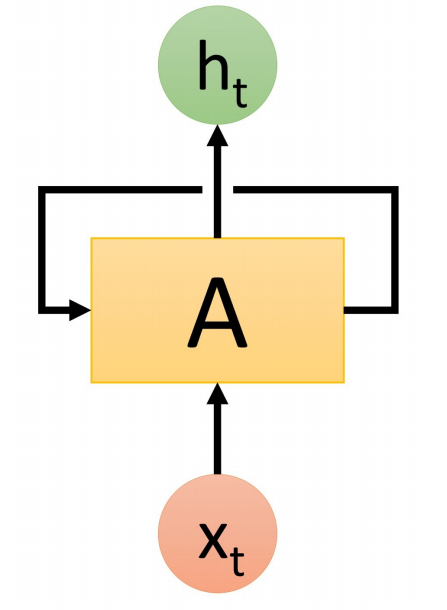
\includegraphics[scale=0.3]{images/chap2_rnn.png}
    \caption{遞迴式神經網路示意圖}\label{fig:chap2_rnn}
\end{figure}
\subsection{簡介}
雖然深層類神經網路擁有很好的分類能力,但是當輸入資料呈現序列狀 (Sequential) ,且有上下文關係 (Context Dependency) 時,如語音辨識 (Speech Recongnition) ,這時候深層類神經網路就無法妥善處理。因此這時候需要記憶細胞 (Memory Cell) 來幫助,即是遞迴式類神經網路,圖 ~\ref{fig:chap2_rnn} 為其架構。不同於深層類神經網路,它是帶有循環的神經網路。在圖 ~\ref{fig:chap2_rnn} 中, $A$ 代表神經網路的主體, $x_t$ 代表在時間點 t 時的輸入, $h_t$ 代表在時間點 t 時的網路輸出,這種循環結構能使資訊從前面傳遞到後面,能夠允許資訊保留一段時間。我們將迴圈展開後,不難發現其可根據輸入之料的序列關係展開成一鏈狀結構,如圖 ~\ref{fig:chap2_unrollrnn} 所示,因此我們可以將遞迴神經網路想像成是有多層相同的神經網路,每一層都會將資訊傳遞給下一層。

\begin{figure}
    \centering
    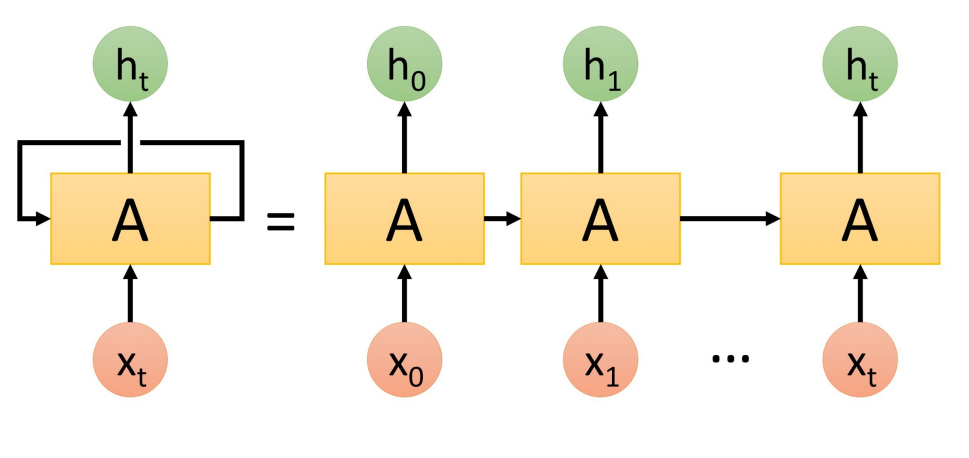
\includegraphics[scale=0.18]{images/chap2_unrollrnn.png}
    \caption{遞迴式神經網路展開示意圖}\label{fig:chap2_unrollrnn}
\end{figure}

%\subsection{沿時間反向傳播演算法 (Backpropagation through Time, BPTT)}
%訓練遞迴類神經網路的方法稱作沿時間反向傳播演算法 ,%TODO
\subsection{長短期記憶神經網絡(Long Short-term Memory Network)}
雖然遞迴類神經網路的設計看起來能有效地處理序列狀的問題,但實作後發現,遞迴類神經網可能會有梯度爆炸或者梯度消失的問題,並無法完美學習長期依賴 (Long-Term Dependencies) ~\cite{bengio1994learning} 。因此人們再度提出一種進階形式:長短期記憶網路 (Long Short-term Memory Network) ~\cite{hochreiter1997long} ,是一種遞迴類神經網路的改善,能夠彌補之前的弱點,學習長期依賴關係。長短期記憶網路如同圖 ~\ref{fig:chap2_unrollrnn} 一般,差別在於 $A$ 架構上的不同,遞迴類神經網路如圖 %TODO ~\ref{fig:chap2_rnnA} 
,僅只有一層 DNN 來更新記憶細胞的值;而長短期記憶網路有三個門閘 (Gate) ,是一種能讓訊息選擇性通過的方式,作為管理單元狀態 (Cell State) 的更新、移除資訊。

我們由左至右來看。首先,先決定哪些資訊需要從單元狀態中拋棄,通過一個遺忘閘 $f_t$ (Forget Gate) 來處理。它接收了現在這個時間點的資訊以及上個時間點的隱藏狀態 (Hidden State) ,分別通過一層線性矩陣轉換投影到同一個維度並相加,再通過一個 S 型函數,成為一個 0 到 1 所組成的向量,如式子(\ref{function:forget}) ,跟 $C_{t-1}$ 來進行逐點乘積 (Pointwise Product) ,因此若 $f_t$ 值為 0 代表要清除之前儲存的內容,而 1 代表完全保留。
\begin{equation}
    f_t = \phi(W_{xf}x_t + W_{hf}h_{t-1} + b_f) \label{function:forget}
\end{equation}

再者,我們需要決定哪些要被儲存進管理單元中,稱為輸入閘 (Input Gate)$i_t$ ,為 S 型函數決定要更新多少資訊,類似遺忘閘 $f_t$ 的概念,如式子 (\ref{function:input_gate})。而至於要更新至管理單元的資訊,則是由另一個非線性函數雙曲正切 (Hyperbolic Tangent, Tanh) 負責產生出候選值 $C_t^{'}$ ,如式子 (\ref{function:candidate}) 。
\begin{equation}
    i_t = \phi(W_{xi}x_t + W_{hi}h_{t-1} + b_i) \label{function:input_gate}
\end{equation}
\begin{equation}
    C_t^{'} = tanh(W_{xC}x_t + W_{hC}h_{t-1} + b_C) \label{function:candidate}
\end{equation}
更新管理單元的方法,只需要將上一個管理單元 $C_{t-1}$ 搭配由雙曲正切產生出的候選值 $C_t^{'}$ ,分別根據 $f_t$ 與 $i_t$ 進行加權和,如此便能更新單元狀態 $C_t$ ,如式子 (\ref{function:update}) 。
\begin{equation}
    C_t = f_t * C_{t-1} + i_t * C_t^{'} \label{function:update}
\end{equation}
最後一個則是輸出閘 (Output Gate) $o_t$ ,跟前兩個門閘一樣,控制多少比例要輸出,如式子 (\ref{function:output}) 。接著管理單元通過雙曲正切函數,使得輸出值介於 -1 到 1 之間,與輸出閘逐點乘積,這樣便可以只更新想要的隱藏狀態,如式子 (\ref{function:hidden_state}) 。

\begin{equation}
    o_t =  \phi(W_{xo}x_t + W_{ho}h_{t-1} + b_o) \label{function:output}
\end{equation}
\begin{equation}
    h_t = o_t * tanh(C_t) \label{function:hidden_state}
\end{equation}

由式子 (\ref{function:forget}) 到 (\ref{function:output}) 可明顯看出,門閘的權值都是由 $x_t$ 和 $h_{t-1}$ 所計算而成。
%TODO GRU
\subsection{序列到序列}
%TODO
%\subsection{位置編碼器 (positional encoding)}
\section{詞彙表示法 - 詞嵌入 (Word Embedding)}
\subsection{基本介紹}
深層學習近年來在自然語言處理領域中已經開拓出越來越大的新空間,而詞嵌入 (Word Embedding) 可說是其中具有相當重要意義的一項工局。傳統上,為了將一個自然語言中所有的詞以數學符號形式呈現,並進行各式自然語言處理問題,最常使用的表達方式是 1-of-N 編碼 (1-of-N Encoding) ,意思是每個詞都被表示成一個維度 $N$ 的詞向量 (Word Vector) , $N$ 為整個詞典的大小,且詞典中的每個詞都對應到一個特定的維度,而一個詞向量只有在該詞所對應到的維度其值為 1 ,其他 $N-1$ 個維度的值都是 0 ,這種表示方式雖然非常的稀疏 (Sparse) ,但其意義卻相當簡潔明瞭, 1 所在的維度即說明了這個詞向量是辭典中的哪個詞,且事實上 1-of-N 編碼在許多問題上,搭配許多機器學習模型進行訓練後都有不錯的表現。

然而 1-of-N 編碼有幾個缺點。首先,由於自然語言辭典 $N$ 的大小一般來說都在數萬至數十萬的量級,因此這種詞向量的維度也非常大,在機器學問題上很容易受到維度災難 (Curse of Dimensionality) 之影響,使表現變差。再者,這種表現方式將詞典中任意兩個詞都視為獨立,完全無法呈現出兩個詞之間的語意關係,就算是兩個同義詞 (Synonym) ,或是詞性變換,他們的 1-of-N 編碼之間也毫無關聯。因此在 1986 年,分佈式表達 (Distributed Representation) 的概念首次被提出,以分佈式表達呈現出的詞向量不僅維度遠低於辭典大小 $N$ ,且每個維度上的值可以是任意的連續實數,所以透過計算兩個向量之間的歐式距離 (Euclidean distance) 或是餘弦相似度 (Cosine Similarity) 之大小,兩者之間的語意關係就能呈現出來,而這些向量所在之空間即稱為語意空間 (Semantic Space) 。此技術產生之詞向量我們將之稱為分佈式詞彙表達法 (Distributed Word Representation) ,或者稱為詞嵌入。

詞嵌入在諸多自然語言處理問題上已經被證明相當有幫助,例如專有名詞辨識 (Name Entity Recognition) 、詞性標註、句法分析 (Syntactic Parsing) 、語意分析 (Semantic Analysis) 、情感分析 (Sentiment Analysis) 、機器翻譯等等。詞嵌入的訓練與抽取方式並不唯一,過去已有眾多方法被研究提出,一種是訓練語言模型 (Language Model) 時所得到的副產物,另一種則是使用特別設計的模型,模擬每個詞與其上下文 (Context) 之間的關係。%由於本論文之研究並未使用前者技術,因此在接下來的段落只會對後者進行詳細介紹。
\subsection{跳躍文法模型 (Skip-gram Model)}
跳躍文法模型 (Skip-gram Model) 是由米式 (Tomas Mikolov) 於 2013 年提出 ~\cite{mikolov2013distributed}~\cite{mikolov2013efficient} ,是一個利用類神經網路來訓練的模型,如圖%TODO
所示,跳躍文法模型可以分為三個層級:

\begin{itemize}
    \item 輸入層:是一個與辭典大小同長度的陣列,採用 1-of-N 編碼形式,而只有該索引的位置之值為 1 ,其餘皆為 0 。此向量用來表示當前詞 $w(t)$ 作為輸入。
    \item 輸出層:每一個矩形都是與辭典大小同長度的陣列,也採用 1-of-N 編碼形式,而只有某一維度的值為 1 ,其餘皆為 0 。不過每一個矩形是代表前後文的詞,例如 $w(t-2)$、$w(t-1)$、$w(t+1)$、$w(t+2)$ ,我們希望透過跳躍文法模型來預測出當前詞的上下文機率分佈。
    \item 隱藏層:通常維度較小,同時也是代表詞向量的維度。代表的是該時間點當前詞 $w(t)$ 透過隱藏層與輸入層之間的一組權重矩陣 $W$ 投影後的向量。和一般類神經網路的隱藏層不同,此投影後的向量不會再通過任何非線性的函數,而投影到 $w(t-2)$、$w(t-1)$、$w(t+1)$、$w(t+2)$ 等所有輸出層之間,都存在一組共享的權重矩陣 $O$ ,把 $w(t)$ 投影後的向量再做一次線性轉換,預測當前這個詞的上下文機率分佈。
\end{itemize}

跳躍文法模型是專為詞嵌入的抽取而設計的模型,而其抽出之詞嵌入即為權重矩陣 $W$ 中的每一行%(Column)
,或換個說法,是 $w(t)$ 經過 $W$ 的投影結果。此模型同樣也是利用反向傳播演算法進行訓練。通常當預測的上下文範圍越大,得到的詞嵌入品質越好,但同時也大幅增加了計算上的複雜度,而且一般來說和當前詞距離越遠的上下文,和當前詞的相關性越低,所以在訓練時,距離越遠的上下文取樣次數會越少,以降低它的影響力。舉例來說,若設定最大上下文的範圍是 $C=5$ ,每次訓練時都會隨機選擇一個數字 $R$ 介於 1 到 C 之間,並且以當前詞過去的 $R$ 個詞至未來 $R$ 個詞,總共 $2R$ 個詞作為模型輸出層要預測的目標。

\section{機器閱讀理解數據集 (MAchine Reading COmprehension, MARCO, Dataset)}
\subsection{語料介紹}
MARCO ~\cite{nguyen2016ms} 是由微軟所提供的
\subsection{問答系統}
問答系統和資訊檢索 (Information Retrieval) 系統最大的不同在於,問答系統只針對使用者輸入的問句回傳對應之答案,而不是提供使用者先關的資訊,讓使用者自己找答案。此種系統的優點是,面對龐大的資料量或者是很多複雜內容的文本時,使用者有時候無法從眾多文字中找出對應的答案,因此問答系統透過文字處理,直接將可能的答案回傳,以方便使用者閱覽。

\chapter{以自動習得之聲學組型加強監督式語意檢索}
  \section{簡介}
本章節以及下一個章節將對於問答系統介紹。在過去,閱讀理解和問答系統已經有很多研究提出模型,如加入專注式機制(Attention Mechanism)或急躁機制(Impatient Mechanism)的模型 \cite{hermann2015teaching} ,試圖想要模仿人類的行為,能忽視其他不重要或無關的輸入,選擇只專注於和需求有關的輸入,此方法最早在視覺圖像領域所提出,目的是希望讓機器學到圖片中所應該專注的物件(Object)或位置,而其成效也已經在圖像領域和機器翻譯中得到證實,如 \cite{mnih2014recurrent} 和 \cite{bahdanau2014neural}。另有加入了記憶(Memory)網路的 Memory Network \cite{weston2014memory} ,可以儲存理解之後的資訊,概念如同 RNN 細胞一般,還有端對端記憶網路(End-to-End Memory Network)\cite{sukhbaatar2015end} ,透過使用回顧式機制,來多次更新記憶。本篇論文使用了專注式機制,來選擇文本的哪些部分該注意,使用記憶網路來儲存相關的文本,並且透過回顧式機制來反覆更新記憶網路。

我們可將整個問答系統分成三個部分,首先針對使用者的查詢詞,透過檢索的方式回傳符合查詢詞的文本。接者,由於回傳的文本過多,因此我們需要一個過濾器(Filter)來判別此文本是否有此查詢詞之答案,以便降低文本的數量。最後在將這些被選出文本與其查詢詞,通過專注式記憶編碼解碼器(Attention-based Memory RNN Encoder-Decoder)\cite{xiong2016dynamic} 抽取出可能的答案,進而回傳給使用者。本論文的檢索部分是採用 Bing 搜尋來取得相關之文本,即為數據集所提供,故本論文僅針對過濾器以及專注式記憶編碼解碼器兩者進行詳細介紹。

在詳細描述模型以前,我們將先簡介機器閱讀理解數據集。 Microsoft 釋出了閱讀理解相關的數據集,而以問答系統來實踐閱讀理解的概念。此數據集約莫有 10 萬筆的問答句以及約 20 萬以上的文章數,對於每個問句,都會有標註此問句的種類,例子如表(\ref{table:query_example} )共 5 類,表(\ref{table:query_percentage})和表(\ref{table:query_type})為機器閱讀理解查詢詞之比例。而 Bing 搜尋針對此問句,會提供大約 8 到 10 個左右的文本段落(Passages),人們再根據這些段落,標註此段落「是否」足夠提供問句之答案,並根據段落給予對應一至多個對應的答案。%cost to get a patent 是被分類為數值(Numeric)、 was ronald reagan a democrat 則是歸類成描述(Description)、diseases caused by clostridium 被歸為名詞(entity)、who was the president who caused the trail of tears 是為人物(Person),而 what sea is iceland in 則為地點(Location)等 5 類,

\begin{table}
    \caption{答案種類例子}
    \label{table:query_example}
    \centering
    \begin{tabular}[h]{|l|l|}
        \hline
        問句類型 & 例子\\
        \hline
        數值(Numberic) & cost to get a patent\\
        \hline
        描述(Description)& was ronald reagan a democrat\\
        \hline
        名詞(Entity) & diseases caused by clostridium\\
        \hline
        人物(Person) & who was the president who caused the trail of tears\\
        \hline
    \end{tabular}
\end{table}

\begin{table}
    \caption{問句包含詞比例}
    \label{table:query_percentage}
    \centering
    \begin{tabular}[h]{|l|l|}
        \hline
        問句包含詞  &百分比\\
        \hline
        what        &42.2\%\\
        \hline
        how         &15.3\%\\
        \hline
        where       &4.4\%\\
        \hline
        when        &2.0\%\\
        \hline
        why         &1.8\%\\
        \hline
        who         &1.7\%\\
        \hline
        which       &1.4\%\\
        \hline
    \end{tabular}
\end{table}

\begin{table}
    \caption{答案種類}
    \label{table:query_type}
    \centering
    \begin{tabular}{|l|l|}
        \hline
        問句類型            &百分比\\
        \hline
        描述 &52.6\%\\
        \hline
        數字    &28.4\%\\
        \hline
        名詞      &10.5\%\\
        \hline
        地點    &5.7\%\\
        \hline
        人物      &2.7\%\\
        \hline
    \end{tabular}
\end{table}

\section{模型架構介紹}
%\subsection{專注式記憶編碼解碼器}
圖(\ref{fig:dmn})為本章節之系統架構圖之一。以下會針對此架構圖做分析。

\subsubsection{位置編碼}
首先每個段落透過 Natural Language Toolkit (NLTK)來做英文句子的斷句,即會得到 $M$ 個句子,每個詞都有一個詞向量 $w_j^i$,其中 $i$ 代表第 $i$ 個句子,而 $j$ 代表第 $i$ 個句子的第 $j$ 個詞,一個句子可以使用 RNN ,或者是詞袋模型(Bag of Word Model, BOW)將其編碼(Encode)成一個句向量(Sentence Vector),而此處則是採用位置編碼(Position Encoding)\cite{sukhbaatar2015end}  ,如式子(\ref{PE}),此處使用位置編碼的原因,一方面若是使用詞袋模型,會少了每個詞在句子上順序的重要性,另一方面,使用 RNN 模型雖然能夠有順序之別,但由於本篇論文模型過於複雜,若是使用 RNN 模型,將分別會有兩層 RNN 來處理詞彙與句子,會容易過度貼合,因此本篇論文採取折衷的方法,是採用位置編碼,可以得到每個句子的句向量 $f_i$ 代表第 $i$ 個句子

\begin{equation}
    f_i = \sum_{j=1}^M l_j \circ w_j^i
\end{equation}
其中 $\circ$ 為逐點乘積,而 $l_j$ 則為
\begin{equation}
    l_{jd} = (1 - \frac{j}{M}) - (\frac{d}{D})(1 - \frac{2j}{M}) \label{PE}
\end{equation}
其中 $d$ 是詞向量的第 $d$ 維, $D$ 是詞向量的維度,$j$ 代表一句話的第 $j$ 個詞。

\begin{figure}[h]
    \centering
    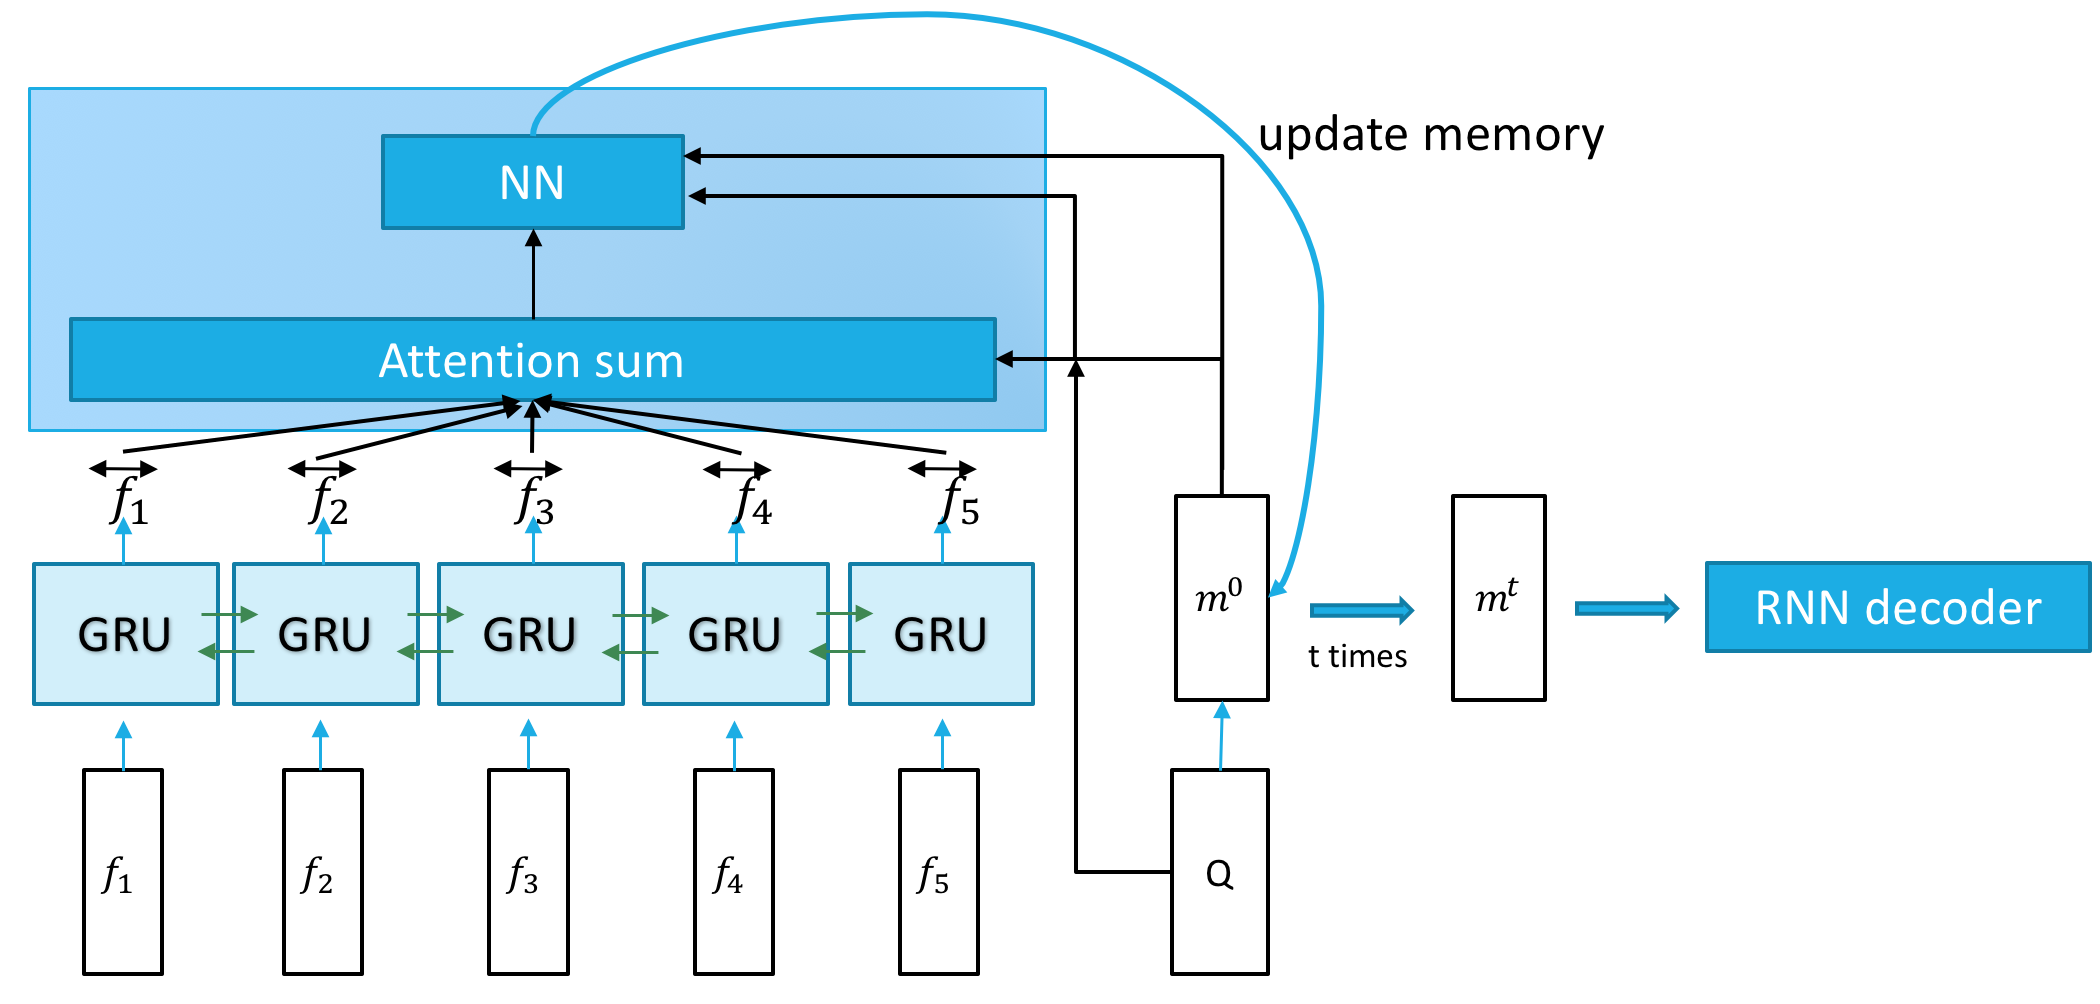
\includegraphics[scale=0.54]{images/chap3_dmn.png}
    \caption{專注式記憶編碼解碼器}\label{fig:dmn}
\end{figure}
\subsubsection{雙向式遞迴式類神經網路}
在得到句向量 $f_i$ 後,為了強化句子與句子彼此之間的關聯性,我們採取了雙向式遞迴式類神經網路(Bidirectional Recurrent Neural Network, BRNN),是由兩個遞迴式類神經網路,一為正向(Forward)遞迴式類神經網路輸出向量表示 $\overrightarrow{f_i}$ ,另一為反向(Backward)遞迴式類神經網路輸出向量表示 $\overleftarrow{f_i}$ ,並且取正向遞迴式類神經網路的第 $i$ 個時間點輸出向量 $\overrightarrow{f_i}$ ,與反向遞迴式類神經網路的第 $i$ 個時間點 $\overleftarrow{f_{M-i}}$ ,並把他們相加起來作為每個句子的向量表示 $\overleftrightarrow{f_i} = \overrightarrow{f_i} + \overleftarrow{f_{M-i}}$ ,即為圖(\ref{fig:dmn})中 GRU 之輸出。雖然採取了雙向式遞迴式類神經網路,但依然容易失去長期的資訊,且我們不僅僅只是要讀過文本而已,我們更需要結合查詢詞來回答問題,因此在此處我們導入了專注式機制的技術。

\subsubsection{專注式機制}
專注式的機制,就是為了比較查詢詞 $Q$ 與文本 $\overleftrightarrow{f_i}$ 之間的相關性,然而專注式機制的實作方法有很多,但核心的概念是為了找尋兩者間之相似性(Similarity),即稱為專注式權重 $\alpha_i$ ,以下是幾種常見計算專注式權重之方法:
\itemsep -4pt
\begin{itemize}
    \item 歐式距離:$\alpha_i = ||Q-\overleftrightarrow{f_i}||_{2}$
    \item 餘弦相似性:
            $\alpha_i = \frac{Q \circ \overleftrightarrow{f_i} }{|Q| |\overleftrightarrow{f_i}| } $ 
            ,其中 $\circ$ 為 逐點乘積
    \item 類神經網路: $\alpha_i = W_a ([Q ; \overleftrightarrow{f_i}]) $ 
        ,其中 $\alpha_i$ 為一純量(Scalar) $;$ 代表串連兩個向量。
\end{itemize}
本論文採取最後一種深度類神經網路的方法,然此處深度神經網路的輸入是為 $z_i$ ,結合句子 $\overleftrightarrow{f_i}$ 、問句 $Q$ 以及記憶 $m$ 表示的資訊,如式子($\ref{function:nninput}$)
\begin{equation}
    z_i = [ \overleftrightarrow{f_i} \circ Q ; \overleftrightarrow{f_i} \circ m ; |\overleftrightarrow{f_i} - Q| ; | \overleftrightarrow{f_i} - m| ] \label{function:nninput}
\end{equation}
其中 $m$ 是經由 $Q$ 來初始化,而 $|\cdot|$ 是向量取絕對值。

接著我們讓 $z_i$ 通過兩層類神經網路,可得一純量 $Z_i$。在得到了專注式權重 $Z_i$ 以後,我們對其做正規化,此處我們選擇「對所有句子的 $\alpha$ 值通過軟性最大化」,通過軟性最大化可以更加強化相關的句子,降低其餘句子的雜訊,如式子($\ref{function:attention}$)。
\begin{equation}
    g_i = \frac{exp{(Z_i)}}{\sum_{k=1}^{M} exp(Z_i)} \label{function:attention}
\end{equation}

結合正規化後的專注式權重 $g_i$ ,我們可對於文章抽取出基於我們想要專注點的語境向量(Contextual Vector),如式子(\ref{function:context_vector})。
%TODO contextual vector 中文
\begin{equation}
    c = \sum_{i=1}^{M} g_i \overleftrightarrow{f_i} \label{function:context_vector}
\end{equation}
%在得到了專注式權重以後,我們需要對其做正規化,
%而本篇論文另外使用了一種計算相似性的方法,
%\itemsep -2pt
%\begin{itemize}
%    \item Stochastic "Hard" Attention
%    \item Deterministic "Soft" Attention
%\end{itemize}
\subsubsection{記憶(Memory)}
在得到語境向量後,下一步則是要更新記憶 $m$ ,與計算專注式的權重一樣,通過一個類神經網路,輸入為當前的記憶、語境向量、以及固定的問句表示,進而更新記憶,如式子(\ref{function:update_memory})。
\begin{equation}
    m = ReLU(W [m; c; Q] +b) \label{function:update_memory}
\end{equation}
\subsubsection{回顧式機制}
在此,我們把計算專注式權重的值以及更新記憶的值,視為一個循環,我們把它稱為一個回顧,每經過一次回顧,相當於是再次讀過句子,重新理解再存入記憶裡,如圖(\ref{fig:dmn})所示,可以更新 t 次。
\subsubsection{解碼器}
最後再用儲存的記憶連接到一個遞迴式類神經網路,以便解碼出可能的答案,如式子 \ref{function:answer_module} ,而損失函數則是每個字的交叉熵。
\begin{equation}
    \label{function:answer_module}
    \begin{aligned}
    a_0 = m \\
    a_t = GRU(y_{t-1}, a_{t-1}) \\
    y_t = softmax(W^{(a)} a_t)
    \end{aligned}
\end{equation}

\section{基本實驗配置}
\subsection{前置處理}
\itemsep -4pt
\begin{itemize}
    \item 前處理:此數據集包含大量的英文,夾雜部分日文以及標點符號,若是選用所有的詞彙(Vocabulary),會有四十幾萬的詞(Word),我們試著降低詞彙的數量,移除掉標點符號和文本中的網址,並把所有英文字母轉成小寫,最後我們把詞彙量降到了約莫 14 萬個詞。
    \item 訓練方法:我們選擇將詞嵌入一併與我們的模型一起訓練。而為了避免過度貼合,對於所有的遞迴式類神經網路,都使用了丟棄演算法,而對於所有的可訓練的(Trainable)權重進行正規化。在回顧機制裡,我們設置回顧次數的範圍在 1 到 3 次。此外我們採用負採樣(Negative Sampling)的技巧,來降低整個模型所需要的參數量。
    \item 衡量標準:本論文對於問答系統所使用的衡量標準是 ROUGE (Recall-Oriented Understudy for Gisting Evaluation)\cite{lin2004rouge} ,常用於摘要(Summarization)或機器翻譯,是一種評比參考(Reference)字串和預測(Prediction)字串之間相似程度的量表,包含基於正確 n-元語法(n-gram)的 ROUGE-1 和 ROUGE-2 ,以及基於最長共同子字串(Longest Common Subsequence)長度的 ROUGE-L。ROUGE 值是一個介於 0 至 1 之間的實數,ROUGE 值表示兩字串的相似度越高。本篇論文採用的是 ROUGE-L 的分數。

\end{itemize}
\subsection{基準實驗}
我們總共提出兩種基準實驗模型,如圖(\ref{fig:baseline1})及(\ref{fig:baseline2})。
圖(\ref{fig:baseline1})先以問句當作編碼器的初始狀態,再將文本依序編碼,再用解碼器產生文字。圖(\ref{fig:baseline2})則是每個句子都和問句串接一起接到編碼器,之後再用解碼器產生文字。兩者的解碼器皆有使用專注式 \cite{bahdanau2014neural} 的技巧。
%TODO describe baseline
\begin{figure}[h]
    \centering
    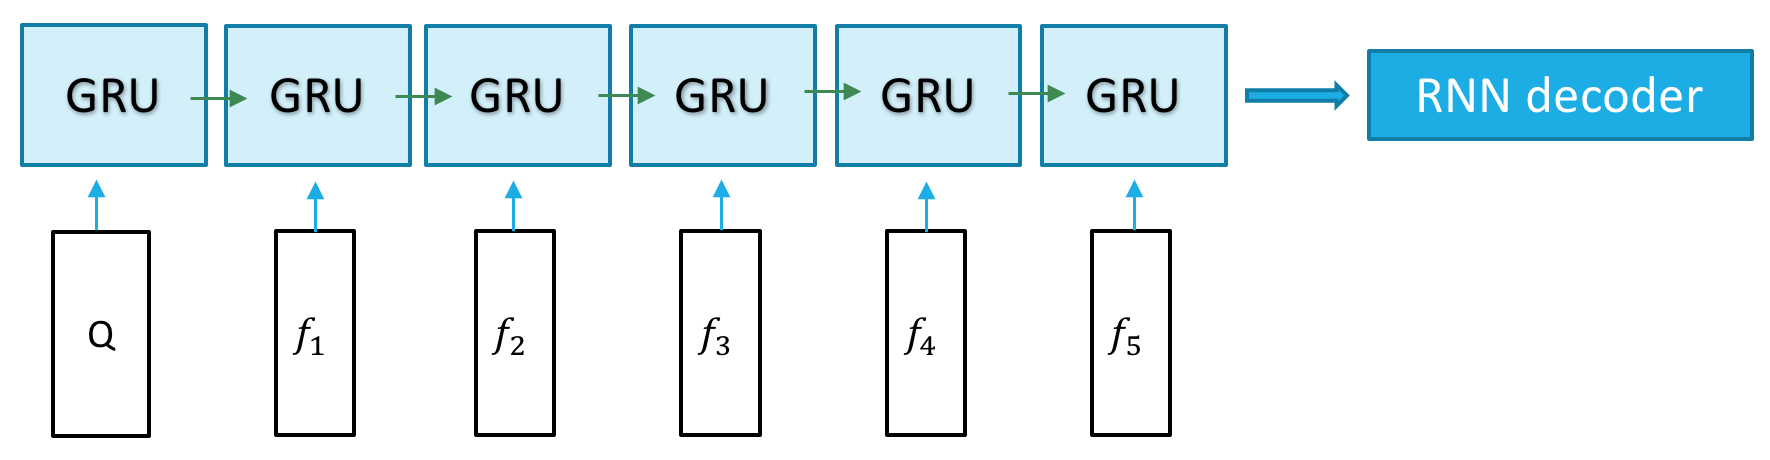
\includegraphics[scale=0.54]{images/chap3_baseline1.png}
    \caption{基準實驗模型一}\label{fig:baseline1}
\end{figure}
\begin{figure}[h]
    \centering
    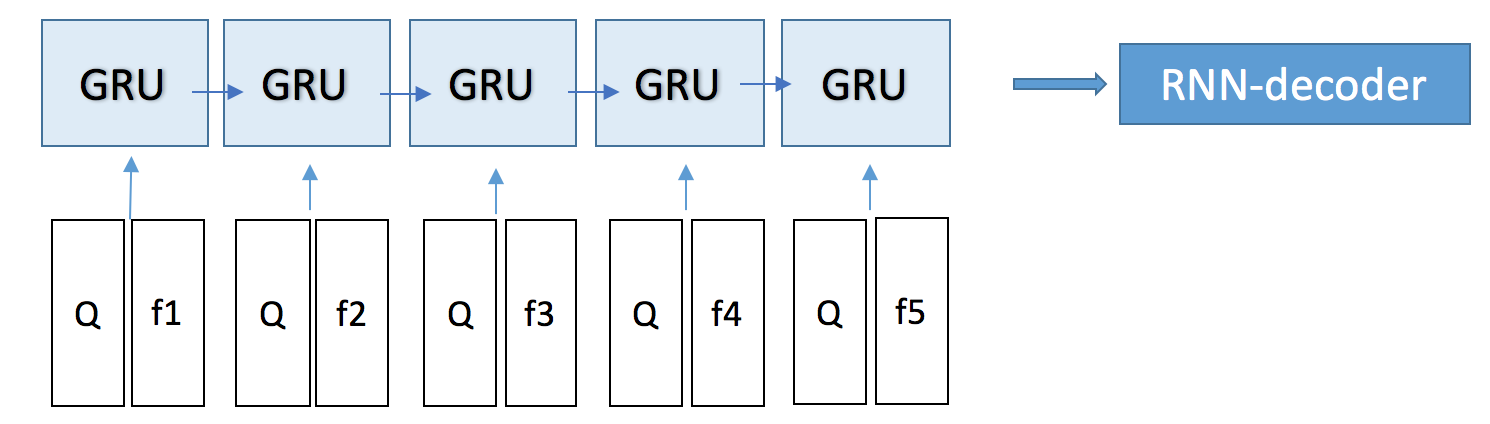
\includegraphics[scale=0.54]{images/chap3_baseline2.png}
    \caption{基準實驗模型二}\label{fig:baseline2}
\end{figure}

\section{實驗結果與討論}
\subsection{記憶細胞大小}
我們分別測試遞迴式網路的大小,分別是 128 、 256 以及 512 ,並試著增加詞向量的空間至 1000 維。
\begin{table}
    \caption{遞迴類神經網路實驗結果}
    \label{table:RNNCell_size}
    \centering
    \begin{tabular}{|l|l|l|}
        \hline
        記憶細胞大小&詞向量 & ROUGE\\
        \hline
        128 & 500 & 33.34\% \\ %Valkyrie\_0 \\
        \hline
        256 & 500 & 33.30\% \\
        \hline
        512 & 500 & 33.95\% \\
        \hline
        512 & 1000 & 33.22\% \\
        \hline
    \end{tabular}
\end{table}
\subsection{回顧次數}
我們在此測試回顧次數對模型之影響的影響。如表 \ref{table:hop} 可見,最佳的情況是發生在兩次的情形。%可能不需要太多次的回顧,甚至有些語意只需要一次便能理解。
\begin{table}
    \caption{回顧次數實驗結果}
    \label{table:hop}
    \centering
    \begin{tabular}{|l|l|}
        \hline
        回顧次數 & ROUGE\\
        \hline
        1 & 33.63\% \\
        \hline
        2 & 33.95\% \\%34426306Valkyrie\_1\\
        \hline
        3 & 33.22\% \\
        \hline
    \end{tabular}
\end{table}
\subsection{取代數字}
另外,為了再降低複雜度,我們特別對阿拉伯數字進行處理,把所有阿拉伯數字取代成特定標籤,或者是以文本數字出現的順序,分別給予數字一、數字二、數字三等等,把詞彙量降低到 13 萬左右。
\begin{table}
    \caption{數字處理}
    \label{table:digit}
    \centering
    \begin{tabular}{|l|l|}
        \hline
        數字取代方法 & ROUGE\\
        \hline
        保留數字 & 24.13\% \\%Caishen\_1 \\
        \hline
        統一所有數字 & 33.68\% \\
        \hline
        數字依文章順序標注 & 33.95\% \\
        \hline
    \end{tabular}
\end{table}
\subsection{模型比較}
由表 \ref{table:model} 可見,基準實驗模型的表現只有 20\% 左右,我們的模型相較之下大幅領先。然而,雖然目前仍無法到達人類的標準,但相信對於問答系統已經是一大突破了。
\begin{table}
    \caption{模型比較}
    \label{table:model}
    \centering
    \begin{tabular}{|l|l|}
        \hline
        模型 & ROUGE\\
        \hline
        基準實驗模型一 & 18.63\% \\
        \hline
        基準實驗模型二 & 22.01\% \\%Venus\_0 \\
        \hline
        ReasoNet Baseline \cite{shen2016reasonet}& 19.20\% \\
        \hline
        FastQA \cite{weissenborn2017making} & 33.67\% \\
        \hline
        專注式記憶編碼解碼器 &  33.95\% \\ %best\_score
        \hline
        Prediction \cite{wang2016machine} & 37.33\% \\
        \hline
        ReasoNet \cite{shen2016reasonet} & 38.81\% \\
        \hline
        R-Net & 42.89\% \\
        \hline
        Human Performance &47\% \\ %TODO 中文
        \hline
    \end{tabular}
\end{table}
\subsection{答案種類比較}
另外針對答案種類我們做了分析,發現數值類的結果明顯比其他四種還要好,而描述類次之,可能原因是數字類的回答敘述較為一致,而描述類包含有些是非題這種簡單容易學習的答案,且此兩者之題型相較其他題型比例亦偏多,模型也因此能夠有較好的表現。%4659,1948,537,154
\begin{figure}
    \centering
    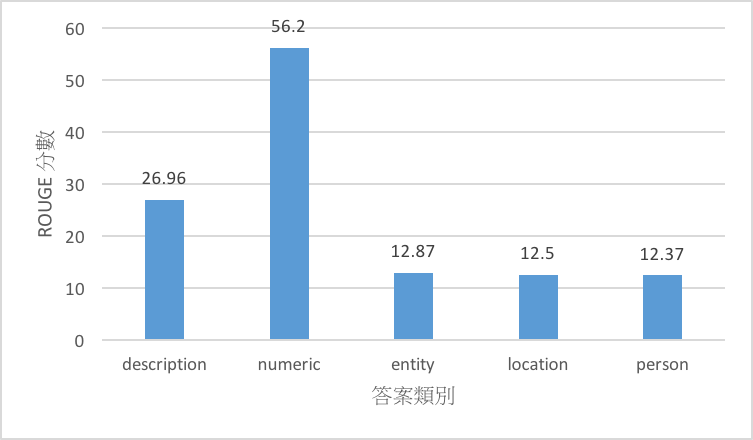
\includegraphics[scale=0.7]{images/chap3_rouge_dist.png}
    \caption{答案種類之 ROUGE 分數}
    \label{fig:rouge_dist}
\end{figure}
%\subsection{更新記憶方法}
\section{範例與分析}
我們挑選幾個專注式機制在不同回顧的次數所專注之表現,如圖 \ref{fig:attn_1} 、 \ref{fig:attn_2} 和圖 \ref{fig:attn_3}。

圖 \ref{fig:attn_1} 的問句為「how many years to become an accountant」,答案為「Four year」,與我們模型產生的句子結果一樣。而看圖可發現回顧三次可以會越來越集中於含有標準答案資訊的句子。再看
圖 \ref{fig:attn_2} ,其問句為「what region is indiana in」,答案為「U.S」,而我們模型產生的是「north county」,雖專注的點正確了,但卻與答案不同,僅僅對了部分的意思,並未提及美國相關的詞,我們進一步觀察到在其他訓練階段所產生的句子有「united states」、「north america」跟「us」等,由此可見,模型應該有學習到答案是「美國」相關的意思。
\begin{figure}
    \centering
    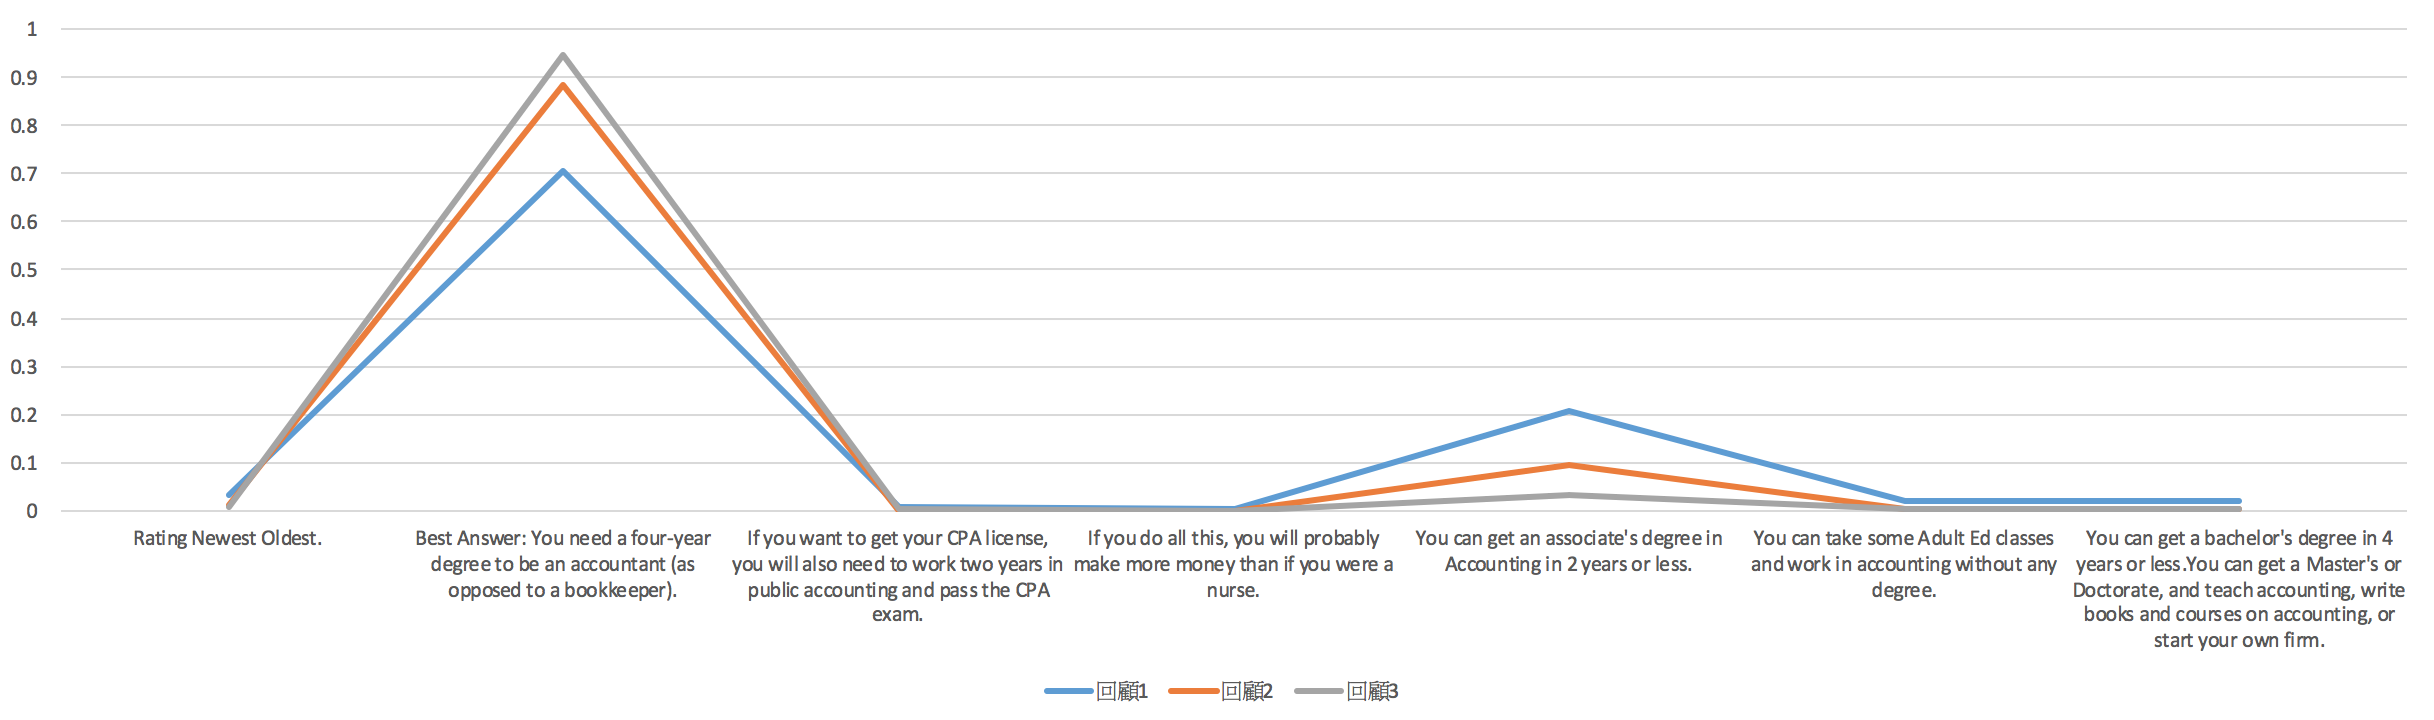
\includegraphics[scale=0.6,angle=90]{images/chap3_attn1.png}
    \caption{專注式結果1}\label{fig:attn_1}
\end{figure}
\begin{figure}
    \centering
    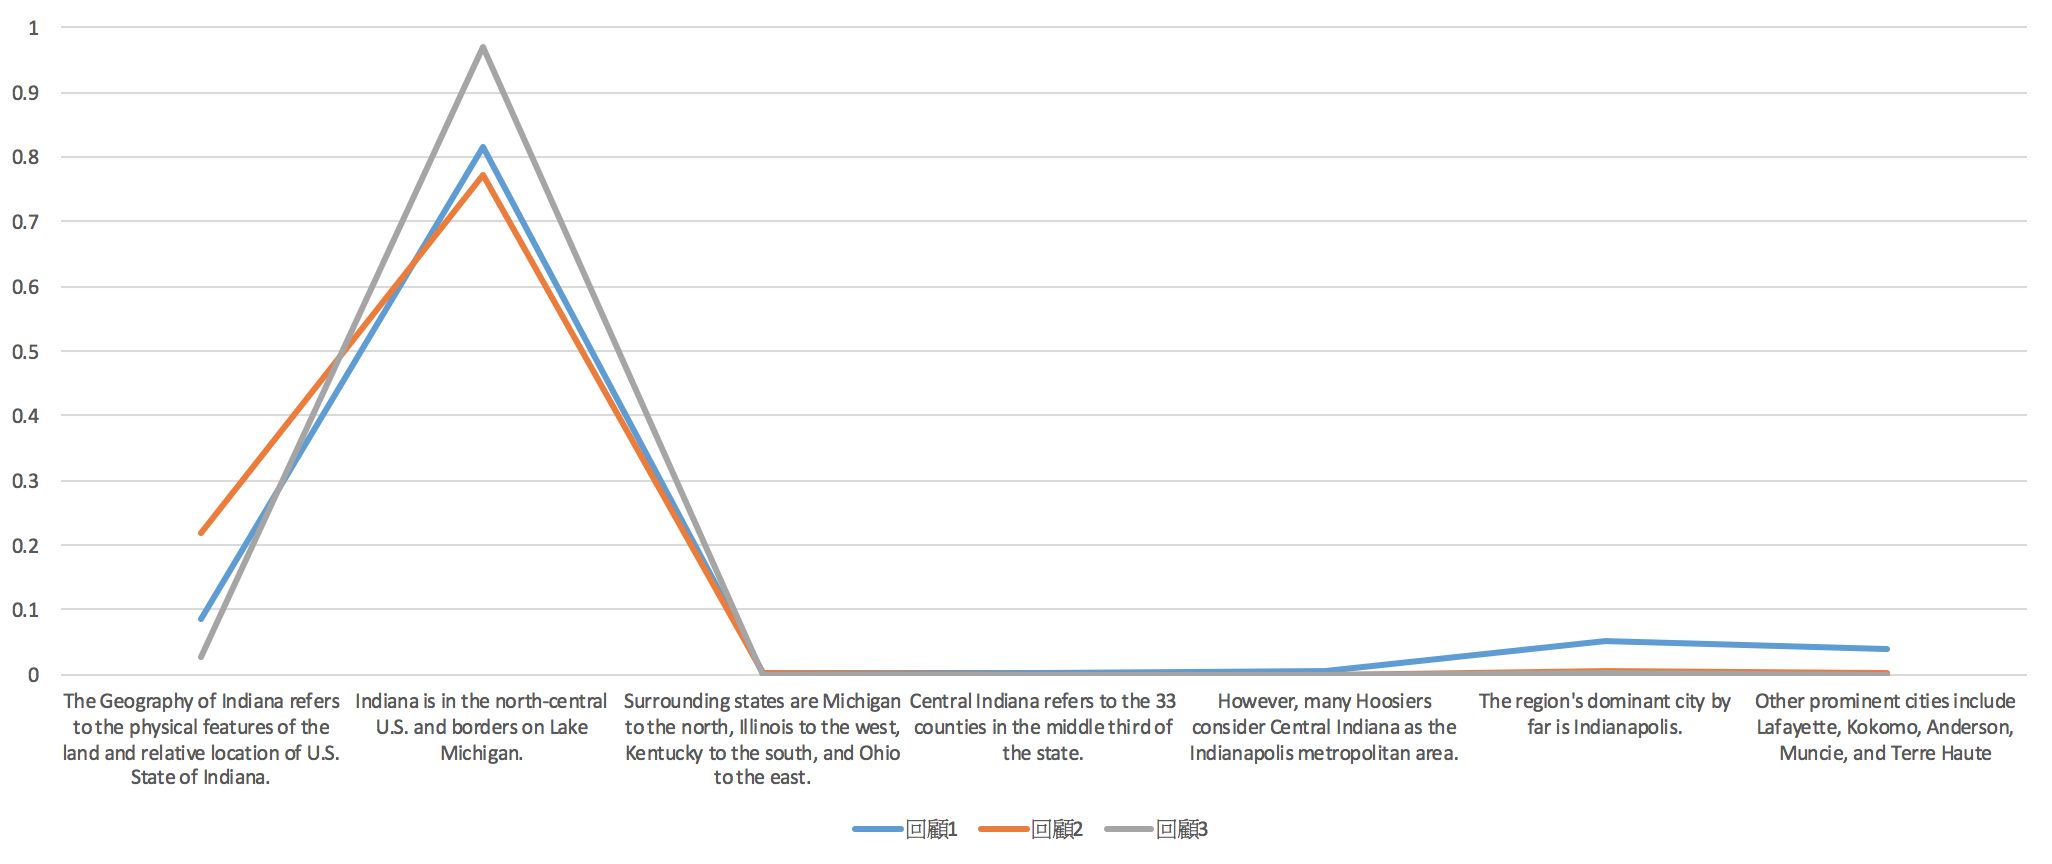
\includegraphics[scale=0.65,angle=90]{images/chap3_attn2.png}
    \caption{專注式結果2}\label{fig:attn_2}
\end{figure}

圖 \ref{fig:attn_3} 為一反例,其問句為「what means irie」,答案是「Alright, powerful and pleasing, excellent, highest, the state of feeling great.」,而我們模型所生成之答案為「comfort」,並無與答案完全一樣的字詞,且其專注點位於第一句「Irie (I rie I '  ree) is the word in Jamaican Patois that means, alright.」,而以我們人類角度來看,與答案有相關的應為第二句「The term can be used to mean 1: powerful and pleasing; 2: excellent, highest; n 3: the state of feeling great.」。
\begin{figure}
    \centering
    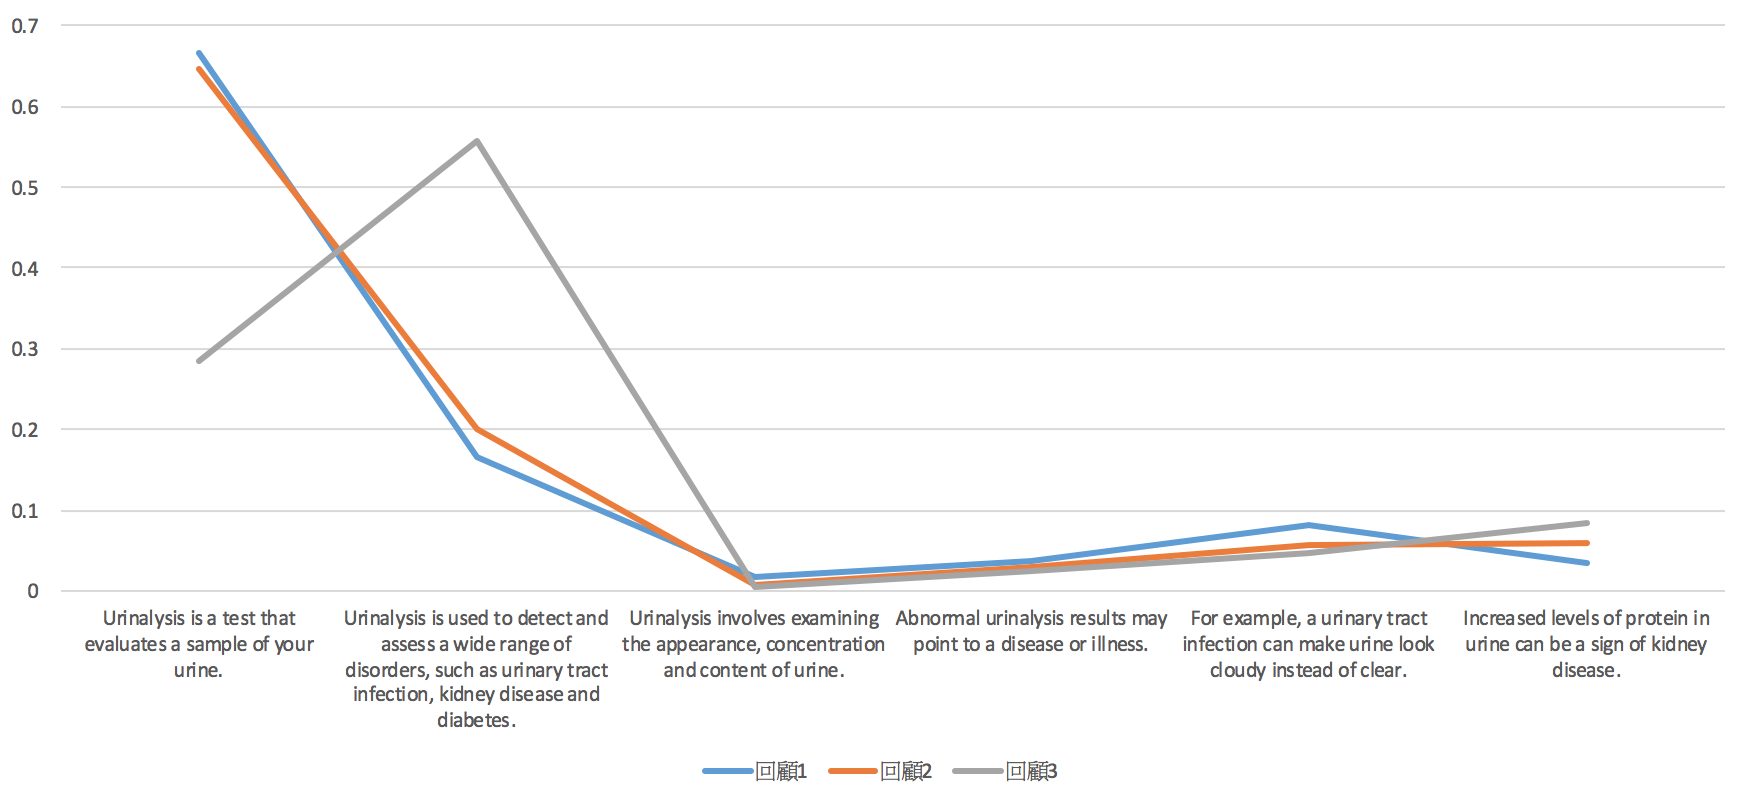
\includegraphics[scale=0.6,angle=90]{images/chap3_attn3.png}
    \caption{專注式結果3}\label{fig:attn_3}
\end{figure}
%\begin{table}
%    \caption{答案種類}
%    \label{table:example}
%    \centering
%    \begin{tabular}{|l|l|l|}
%        \hline
%        問句 & 參考答案 & 模型答案\\
%        \hline
%        what means irie & Alright, powerful and pleasing, excellent\\, highest, the state of feeling great. & comfort \\
%        \hline
%    \end{tabular}
%\end{table}
%TODO analysis weight
\begin{figure}
\end{figure}
\section{本章總結}
在本章節我們試著針對問句與其對應之文本,來產生可能之答案,可見我們在限制領域裡,已經能有不錯的表現,達到 33.95 \% ,雖然有些模型的表現比我們的模型好,但此處我們的方法並不僅僅侷限於文章中的抽取,而是靠著機器產生出最可能的句子。然而,要能夠回答更廣泛的問題,我們需要有效的方法,找出可能含有答案的文本,這部分我們將在第四章介紹。另外,我們發現對於要回答過長的句子,失真的可能性相當高,對此解決方法,我們將在第五章介紹。
%從實驗當中可以發現,我們已經不難從單一文本之中產生答案,然而
%雖然機器可以回答出部分的正確問題,但在此處我們是基於特定文本,以期望機器給予正確回答,但現實情況中,我們必須基於大量的資訊,因此我們要試著從大量的資訊中挑選出相關的文本,能使我們的模型更加有用。

\chapter{以自動習得之聲學組型實現非監督式語意檢索}
  \section{簡介}
接續前一章所提到,我們需要使用一個過濾器,從檢索的回傳值中挑選出最可能含有答案的文本。困難的點在,這並非僅僅是找尋文本中是否包含有查詢詞,因為這在檢索時已經使用過了。更深入的是,我們需要能夠判別語意是否能夠回答到查詢詞。故在此若僅只是使用詞頻(Term Frequency,tf)—逆向檔案頻率(Inverse Document Frequency,idf),對於要選擇出是否包含著答案的文本並不容易。對此,我們使用了相同的模型來解決這件事情,差別僅僅是把編碼器編碼後的結果,通過一層分類器來判別文本是否有包含查詢詞,如圖(\ref{fig:classifier})%TODO
\section{基本實驗配置}

\chapter{利用遞迴式類神經網路語言模型加強非監督式語音文件檢索}
  \section{簡介}
由於模型過於複雜,對於解碼器而言所產生的句子容易出現重複的字,並不明顯合乎語言模型(Language Model)的句子,為了解決這個問題,我們打算分開解碼器模型的部分,事先訓練好一個解碼器,以減少重複字出線的狀況。
\section{變分遞迴式自動編碼器}
我們採用隨插即用(Plug and Play)\cite{nguyen2016plug} 的概念,我們先針對在解碼器的部分,我們採用預訓練(Pre-train)的方法。首先訓練一個自動編碼器(AutoEncoder),此自動編碼器結合遞迴式類神經網路 \cite{bowman2015generating} 和變分(Variational)的方法,稱為變分遞迴式自動編碼器(Variational Recurrent AutoEndoder),再將訓練好的自動編碼器只取其解碼器的模型,接回專注式記憶編碼解碼器,來達到更好的成效。
\begin{figure}[h]
    \centering
    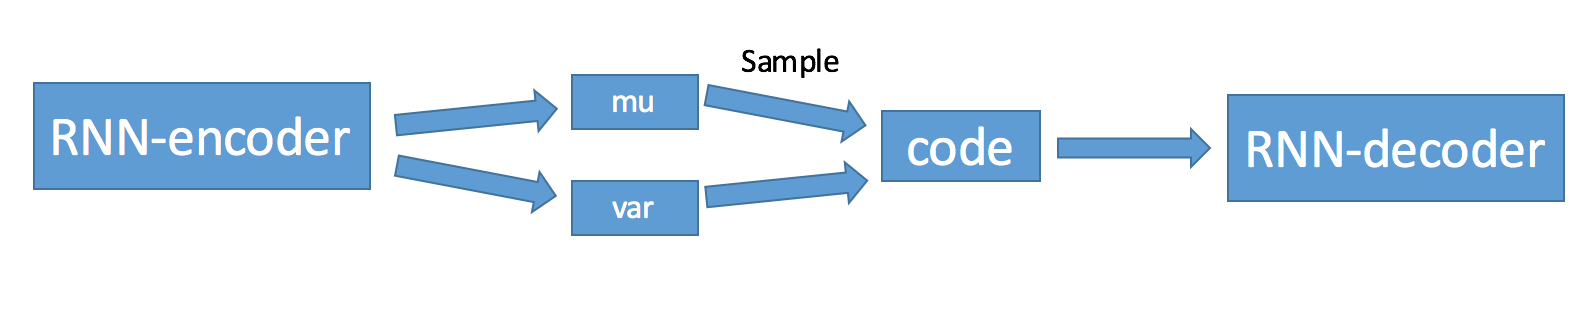
\includegraphics[scale=0.52]{images/chap5_vrae.png}
    \caption{變分遞迴式自動編碼器}\label{fig:vrae}
\end{figure}
\subsection{遞迴式自動編碼器}
遞迴式自動編碼器與自動編碼器的概念相似,差別是在潛在向量(Latent Vector)的編碼方式是透過遞迴式類神經網路來取得,也用遞迴式網路來重建句子。
\subsection{變分機制}
我們對遞迴式自動編碼器的部分加入了變分機制,如圖(\ref{fig:vrae}),編碼器降維到一個潛在空間(Latent Space)$q_\theta(z|x)$ ,其中 $\theta$ 代表編碼器的參數(Parameter)。 編碼後的結果去得到平均值 $\mu$(Mean)與變異數 $\sigma$(Variance),並能得到基於編碼器所形成的分佈 (Distribution)。
之後在用 $q_\theta(z|x)$ 來取樣(Sample)出潛在變量 $z$(Latent Variable),如式子(\ref{function:sample})。
%$p_\phi(x|z)$而這個分佈的平均值是 0 ,而變異數是 1 ,如式子 \ref{function:prob},並由此分佈來取樣(Sampled)出潛在變量(Latent Variable),如式子\ref{function:sample} ,當作解碼器的初始狀態(Initial State)。
\begin{equation}
    z = \mu + \sigma \odot \epsilon \label{function:sample}
\end{equation}
其中 $\epsilon \sim Normal(0,1)$ 。

以潛在變量當作解碼器的初始狀態,以此來重建(Reconstruct)回原來的句子,在此以 $p_\phi(x|z)$ 表示,$\phi$ 代表解碼器的參數。
%\begin{equation}
%    q_\theta(z|x) p(z)
%    p_\phi(x|z)
%    \label{function:prob}
%\end{equation}
這時候,問題就變成要讓 $q_\theta(z|x)$ 接近高斯分佈(Gaussian Distribution)以及能重建回輸入的準確率。要讓此分佈趨近高斯分佈,我們靠得是克雷散度(Kullback–Leibler Divergence)。
\subsection{克雷散度}
克雷散度是用以衡量兩組機率分佈的距離,值越大則代表兩組分佈越不相似。我們試著衡量編碼器的分佈 $q_\theta(z|x)$ 與 $p(z)$ ,衡量兩者之間有多相似,如式子(\ref{function:KL})。
\begin{equation}
    -D_{KL}(q_\phi(z|x)|| p_\theta(z) ) = \frac{1}{2} \sum(1+\log(\sigma^2) - \mu^2 - \sigma^2)
    \label{function:KL}
\end{equation}
其中$p(z)$ 在變分自動編碼器裡為標準常態分佈(Standard Normal Distribution)。
\subsection{損失函數}
整個變分遞迴式自動編碼器模型的損失函數,是由一般遞迴式自編碼器加上正規化所組成,如式子(\ref{function:vrae_loss})。
\begin{equation}
    C(\theta, \phi) = -E_{q_{\theta}}[\log p_\phi(x|z)] + KL(q_\theta(z|x) \| p(z))
    \label{function:vrae_loss}
\end{equation}
第一項代表重建損失(Reconstruct Loss),若無法完整重建句子,則該值會很大。
而第二項則代表編碼器所產生的潛在變量 $z$ 與標準常態分佈之間的差距,該項代表的意義是為了讓潛在變量保持夠多樣(Diverse),例如代表兩個相似意思的句子,在潛在空間裡應該要相近。在此處,我們給予克雷散度一個最低限度,因為 KL 項相較第一項而言容易趨近於 0 ,且容易訓練,但我們最主要的目的是為了重建完整的句子,因而在此處我們給他最低的 KL 值 4 ,讓整個損失函數不置於過度貼合。
%z∼qϕ(z|x)
%$z ~ N(z_{mean}, np.exp(z_{log_{sigma}})^{2})$

%qϕ(z|x) , x̃ ∼pθ(x|z)
%KL divergence
%% Lower bound KL: 4
%difficulty
%% overfit
%variational
\section{實驗結果與討論}
\subsection{變分遞迴式自動編碼器實驗}
%TODO
在變分遞迴式自動編碼器的結果,我們測試重建之結果,在「Yes」、「No」、「approximately \$15,000 per year」等的這種簡短的句子中,都能準確的重建出句子,但若是較長的句子,如「by an infection of oil glands in the eyelid」,仍不是特別理想,僅只能重建成「a infection of infection」。或許若是有足夠的訓練資料,會有更好的表現,如圖 \ref{fig:chap5}。
\begin{figure}
    \centering
    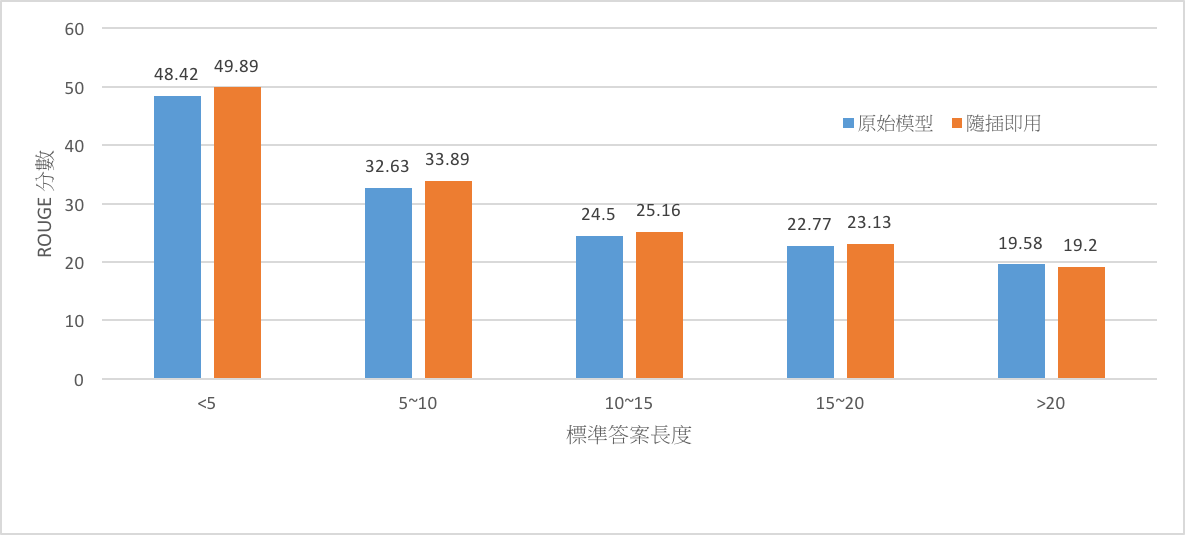
\includegraphics[scale=0.7]{images/chap5.png}
    \caption{針對答案長度分析}\label{fig:chap5}
\end{figure}
\subsection{問答系統模型結果}
在此,我們對訓練好的解碼器,測試與原先的模型比較,以及對解碼器微調(Fine Tune)後的結果來分析。如表 \ref{table:vrae} 所見,我們可發現,在無微調前,直接使用預先訓練好之解碼器,所得到的結果比最初的模型結果還差;然而,若是把解碼器跟著專注式記憶編碼解碼器一起進行訓練、微調,能夠使我們的模型更加進步。%能得到我們目前模型最好的結果。
\begin{table}[ht]
    \caption{採用變分遞迴式自動編碼器之結果} 
    \label{table:vrae}
    \centering
    \begin{tabular}{|l|l|}
        \hline
        模型架構 & ROUGE\\
        \hline
        原始模型 & 33.95\%\\
        \hline
        無微調 & 15.56\%\\%1974768\\
        \hline
        微調 & 34.32\%\\%\\
        \hline
    \end{tabular}
\end{table}
% VRAE loss
%fine tuning or not
\section{本章總結}
隨插即用的方法在生成對抗網路(GAN, Generative Adversarial Network)被使用,而我們將此概念移植至我們的實驗當中,亦能獲得進步,代表預先訓練好一個模型,降低模型訓練的難度,利用隨插即用的技術,能夠讓整體模型更好訓練,亦有更好的表現。%故若是能有更好的解碼器,應該會有更好的結果。

\chapter{在Google Glass上實作個人化的語音翻譯與新聞檢索系統}
  \section{結論}
本碩論主要目的是要透過閱讀文章以及問句,來產生出相對應的答案。過去的問答系統有的是選項式的問答,我們並無法直截了當的知道機器究竟學習到的內容。另外有些是採用大量的自然語言處理分析,抽取出文章內可能句子的段落,然而若是答案並非直接在文章內部,可能無法有效的抓取出答案。在此,藉由類神經網路的方法,
%ROUGE 不一定好
%TODO
\section{未來研究方向}
%加入RL技術,Ensemble, abstract
%TODO

\chapter{結論與展望}
  \input{chapters/chapter7}

\input{thesis_backpages.tex}

\clearpage % to make sure all CJK characters are processed
\end{CJK}  %%% ZZZ %%%
\end{document} 
 
